\chapter{State of the Art} \label{chap:ch3}
\paragraph{}

This chapter reviews the state of the art in MAPF, focusing on the main coordination paradigms and algorithmic approaches proposed in the literature. Section~\ref{sec:mapf_paradigms} surveys decentralized, centralized, hybrid, and learning-based coordination strategies, highlighting their respective strengths and limitations in multi-robot systems. Section~\ref{sec:agent_prioritization} examines agent prioritization heuristics for sequential MAPF planners, with particular attention to their impact on solution feasibility and performance. Finally, Section~\ref{sec:criis_architecture} presents the CRIIS fleet coordination system, which operationalizes centralized MAPF planning and serves as the base for the methods investigated in this work.

\section{Algorithmic Approaches to MAPF}
\label{sec:mapf_paradigms}
\hspace{\parindent}
The MAPF problem has been addressed through different coordination paradigms, reflecting distinct
assumptions about system architecture and the distribution of coordination responsibilities.
In multi-robot systems and fleet coordination, these paradigms exhibit characteristic trade-offs
in terms of coordination quality, computational complexity, and robustness.

This chapter considers the following coordination paradigms:
\begin{itemize}
    \item \textbf{Decentralized coordination};
    \item \textbf{Centralized coordination};
    \item \textbf{Hybrid coordination};
    \item \textbf{Learning-based coordination}.
\end{itemize}

The following subsections discuss each of these paradigms in turn, introducing their main coordination principles and presenting representative algorithmic approaches to illustrate how these paradigms are realized in practice, with particular emphasis on centralized approaches, which constitute the algorithmic focus of this document.

\subsection{Decentralized Coordination}
\label{subsec:decentralized_mapf}
\hspace{\parindent}
Decentralized approaches distribute planning and decision-making among the agents themselves, without relying on a global coordination authority. In this paradigm, agents typically operate based on local information and, when available, limited communication with neighboring agents. Coordination emerges through local interactions, reactive behaviors, or distributed decision-making mechanisms, as illustrated in Figure~\ref{fig:decentralized_architecture}.

\begin{figure}[H]
    \centering
    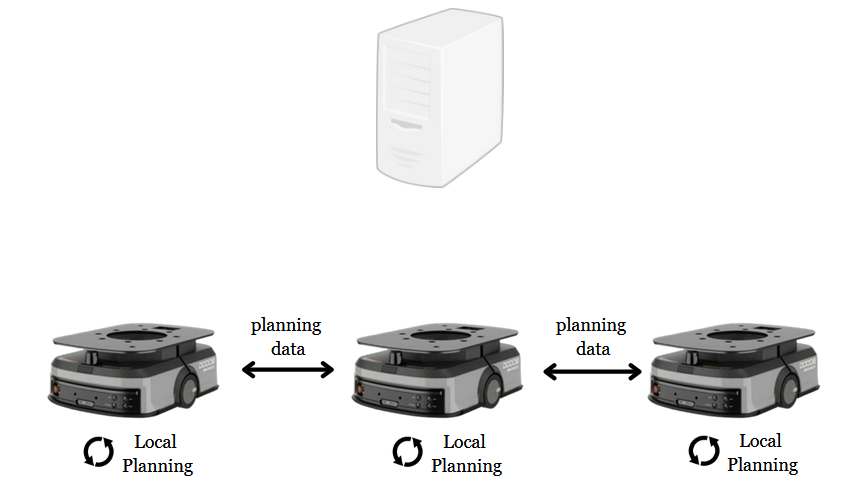
\includegraphics[width=0.8\textwidth]{decentralized_architecture}
    \caption{Illustration of a decentralized coordination architecture, where agents communicate directly with each other and no central planning entity is responsible for computing globally consistent paths.}
    \label{fig:decentralized_architecture}
\end{figure}

Such approaches are particularly attractive in large-scale systems or in scenarios where communication is unreliable, as they avoid centralized computational bottlenecks and single points of failure \cite{siefke2020systems}. Decentralized coordination has been extensively studied in the context of autonomous mobile robots, where agents must operate under partial observability and limited global knowledge \cite{flocchini2000distributed}.

However, the absence of a global planning entity makes it difficult to ensure globally consistent behavior. Decentralized MAPF approaches generally provide limited guarantees with respect to completeness, deadlock avoidance, or solution quality, especially in environments with narrow passages or strong agent interactions \cite{cap2015multi}. As a result, while decentralized paradigms offer scalability, they often struggle to meet the predictability and safety requirements of tightly coordinated robotic fleets.


Several algorithmic approaches exemplify decentralized coordination in multi-robot systems. 
Reactive collision avoidance methods rely exclusively on local sensing and agent--agent interactions to prevent collisions, enabling scalable coordination without global planning, although with limited guarantees \cite{van2008reciprocal}. 
Distributed planning and negotiation-based approaches further extend this paradigm through peer-to-peer information exchange and local conflict resolution, improving robustness while avoiding centralized control \cite{cap2015multi}.


A representative example of decentralized coordination is provided by Artificial Potential Field (APF) methods. Originally proposed for single-agent navigation, APF approaches were designed to guide an agent towards a goal while avoiding obstacles by defining attractive and repulsive potential functions over the workspace \cite{khatib1986real}.
More recent extensions have adapted APF-based methods to multi-robot settings by incorporating interaction forces between agents, which are treated as dynamic obstacles or sources of repulsive potentials. In such approaches, coordination emerges from local interactions, as each agent computes its motion based solely on locally available information. An example of this paradigm is the APF-CPP approach proposed by Wang et al.~\cite{wang2021apf_cpp}, where artificial potential fields are used for online multi-robot coverage path planning in a fully decentralized manner.

The resulting motion emerges from the combination of attractive forces towards goals and repulsive forces arising from obstacles and neighboring agents, allowing agents to react continuously to their local environment without requiring global coordination, as illustrated in Figure~\ref{fig:apf_overview}\subref{fig:apf_forces}.

Although Figures~\ref{fig:apf_overview}\subref{fig:apf_global_minimum} and~\ref{fig:apf_overview}\subref{fig:apf_local_minima} do not explicitly represent a multi-agent setting, they are highly illustrative of the fundamental behavior of potential fields and the emergence of local minima.
Figure~\ref{fig:apf_overview}\subref{fig:apf_global_minimum} depicts an idealized potential field, however, the interaction between attractive and repulsive potentials often gives rise to undesired local minima, as shown in Figure~\ref{fig:apf_overview}\subref{fig:apf_local_minima}. These local minima constitute a well-known limitation of APF-based methods, as agents may become trapped despite the existence of a feasible path to the goal \cite{wu2017apf_annealing}.

\begin{figure}[H]
    \centering
    \begin{subfigure}[t]{0.27\textwidth}
        \centering
        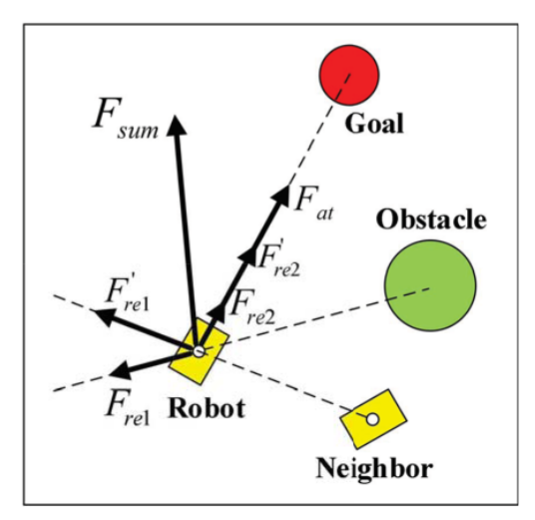
\includegraphics[width=\textwidth]{apf_forces}
        \caption{Attractive and repulsive forces acting on an agent in a multi-robot setting \cite{wang2021apf_cpp}.}
        \label{fig:apf_forces}
    \end{subfigure}
    \hspace{1.0em}
    \begin{subfigure}[t]{0.30\textwidth}
        \centering
        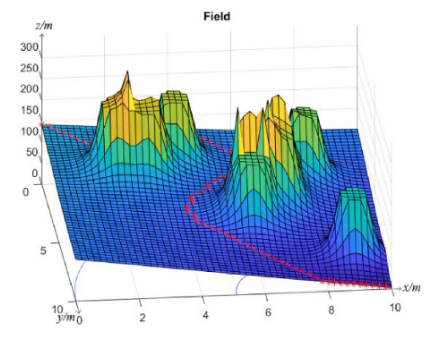
\includegraphics[width=\textwidth]{apf_global_minimum}
        \caption{Potential field \cite{wu2017apf_annealing}.}
        \label{fig:apf_global_minimum}
    \end{subfigure}
    \hspace{0.7em}
    \begin{subfigure}[t]{0.35\textwidth}
        \centering
        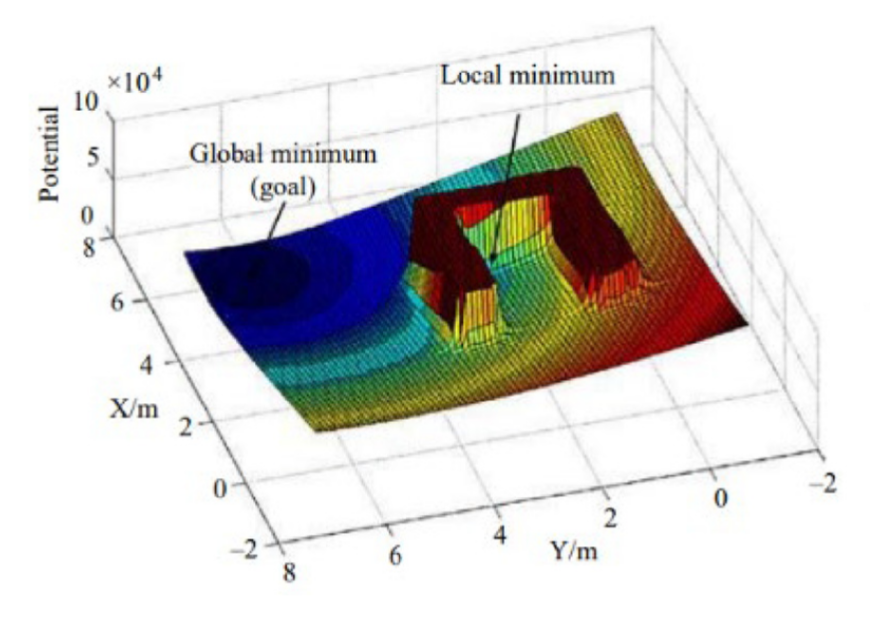
\includegraphics[width=\textwidth]{apf_local_minima}
        \caption{Potential field exhibiting local minima induced by obstacles \cite{wu2017apf_annealing}.}
        \label{fig:apf_local_minima}
    \end{subfigure}
    \hfill

    \caption{Illustration of APF concepts.}
    \label{fig:apf_overview}
\end{figure}


Overall, the APF-based approach discussed above illustrates well several characteristic limitations of decentralized coordination methods. In particular, the reliance on local and reactive decision-making can lead to undesired behaviors such as local minima and deadlocks, reflecting the difficulty of achieving globally consistent solutions. As a result decentralized approaches  typically provide limited guarantees regarding global completeness or solution quality.


\subsection{Centralized Coordination}
\label{subsec:centralized_mapf}
\hspace{\parindent}
Centralized MAPF approaches rely on a single planning entity with access to the complete global state of the system, including the environment representation and the start and goal locations of all agents. This entity is responsible for computing coordinated, collision-free trajectories that ensure globally consistent behavior across the fleet. A typical centralized coordination architecture is depicted in Figure~\ref{fig:centralized_architecture}.

\begin{figure}[H]
    \centering
    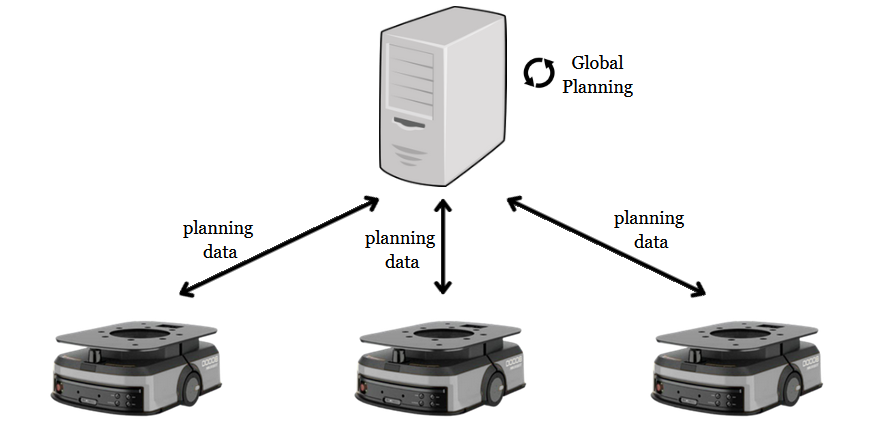
\includegraphics[width=0.8\textwidth]{centralized_architecture}
    \caption{Illustration of a centralized coordination architecture, in which a central planning entity computes coordinated, collision-free trajectories for all agents based on complete global information.}
    \label{fig:centralized_architecture}
\end{figure}


Centralized coordination has long been adopted in industrial and structured environments, where reliable communication and centralized supervision are available \cite{caloud1990indoor}. This paradigm enables strong guarantees regarding safety, predictability, and coordination quality, and aligns well with fleet management systems that incorporate execution monitoring and replanning capabilities.

From a computational perspective, centralized MAPF approaches face inherent scalability challenges as the number of agents increases. As discussed in the background, the MAPF problem is NP-hard under standard formulations, which implies that planning rapidly becomes computationally expensive in densely populated or highly constrained environments. Consequently, practical centralized planners must carefully balance solution quality with computational efficiency. Nevertheless, access to complete global information allows centralized methods to reason explicitly about agent interactions and to resolve conflicts in a systematic and predictable manner, which remains a key advantage in scenarios requiring strong coordination guarantees.


Several algorithmic approaches have been proposed for centralized MAPF planning, differing in how conflicts are represented, detected, and resolved. Throughout this subsection, the discussion focuses on two representative methods, TEA* \cite{santos2016tea} and Conflict-Based Search (CBS) \cite{sharon2015conflict}, which exemplify distinct strategies for centralized coordination.




\subsubsection{TEA*}
\label{subsubsec:tea_star}
\hspace{\parindent}
TEA* is a centralized multi-robot coordination approach that builds directly upon the classical A* search algorithm described in the background by extending the search space with an explicit temporal dimension. Instead of reasoning solely over spatial states, TEA* models robot motion in a space--time representation, where each state is augmented with a discrete time index, enabling the planner to reason explicitly about future agent positions and to avoid conflicts \cite{santos2016tea}.

In this formulation, time progresses in discrete steps that correspond to the traversal of graph edges. Each feasible motion between two adjacent spatial nodes induces a transition to the next temporal layer, and the search is propagated forward up to a predefined temporal horizon \(k_{\max}\). This layered space--time graph, illustrated in Figure~\ref{fig:tea_star_spacetime}, allows TEA* to encode both spatial feasibility and temporal ordering directly within the search process. By reserving nodes and edges across successive time layers during planning, the algorithm ensures that agents do not occupy the same resource at the same time, preventing future conflicts a priori rather than detecting and resolving them after paths have been computed.

\begin{figure}[H]
    \centering
    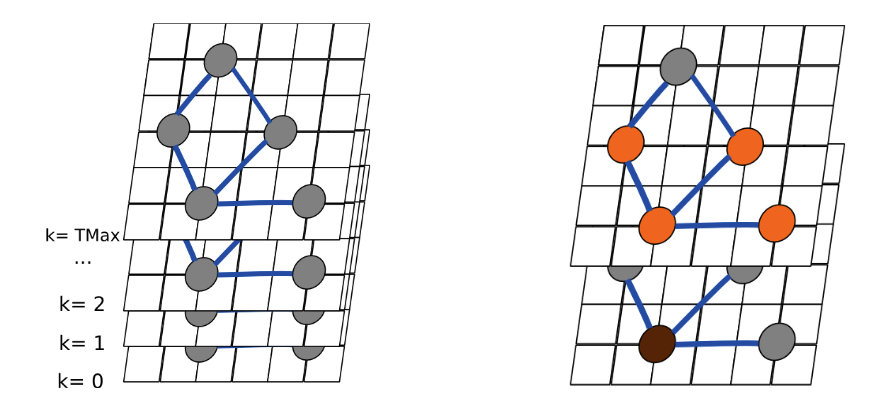
\includegraphics[width=0.85\textwidth]{tea_star_spacetime}
    \caption{Illustration of the TEA* space--time representation \cite{santos2015validation}.}
    \label{fig:tea_star_spacetime}
\end{figure}

In TEA*, paths are planned sequentially for each agent over a shared environment representation, which is commonly modeled as a graph. Once a path is computed for a given agent, the corresponding space--time trajectory is reserved and effectively treated as a dynamic obstacle for subsequently planned agents. During planning, nodes and edges occupied at specific time steps are marked as unavailable, preventing later agents from generating paths that would conflict with already planned motions. This temporal reservation mechanism allows TEA* to generate collision-free solutions, without requiring an explicit conflict detection and resolution stage \cite{santos2015validation}.


A key characteristic of TEA* is its suitability for online execution and replanning. By maintaining a time-indexed representation of resource usage, the planner can update or recompute paths in response to execution delays, dynamic disturbances, or unexpected agent behavior. This capability makes TEA* particularly attractive for industrial and warehouse environments, where strict coordination requirements coexist with execution uncertainty and frequent replanning needs \cite{santos2016tea}.

Several extensions of the original TEA* formulation have been proposed to address limitations arising from simplifying assumptions in the base model. In particular, Moura et al.~\cite{moura2019temporal} introduce a temporal optimization that accounts for robot kinematics, such as orientation changes and rotation costs, reducing the mismatch between the discrete planning model and real-world execution for differential-drive robots. Other works address livelock and deadlock phenomena by dynamically adjusting planning priorities or reordering the sequence in which agents are replanned \cite{santos2015validation}.

Overall, the sequential nature of TEA* implies that the resulting solution may depend on the order in which agents are planned, potentially affecting solution quality or feasibility in densely constrained environments. This limitation, however, can be mitigated through the adoption of appropriate planning heuristics and agent ordering strategies. While this design choice sacrifices optimality guarantees under standard MAPF cost formulations, it offers a favorable trade-off in terms of computational efficiency.

\subsubsection{CBS}
\label{subsubsec:cbs}
\hspace{\parindent}
CBS is a centralized MAPF algorithm that resolves coordination through a hierarchical planning framework composed of a high-level conflict resolution process and a low-level path planner \cite{sharon2015conflict}. The key idea underlying CBS is to decouple individual path planning from conflict management, allowing agents to plan largely independently while explicitly resolving interactions when conflicts arise.

Figure~\ref{fig:cbs_overview}\subref{fig:cbs_problem} illustrates a simple MAPF instance in which two agents navigate a shared environment with alternative routes between start and goal locations. Although individual shortest paths may exist for each agent, conflicts can arise when agents attempt to occupy the same location or traverse the same edge at the same time, motivating the need for explicit coordination.

\begin{figure}[H]
    \centering
    \begin{subfigure}[t]{0.48\textwidth}
        \centering
        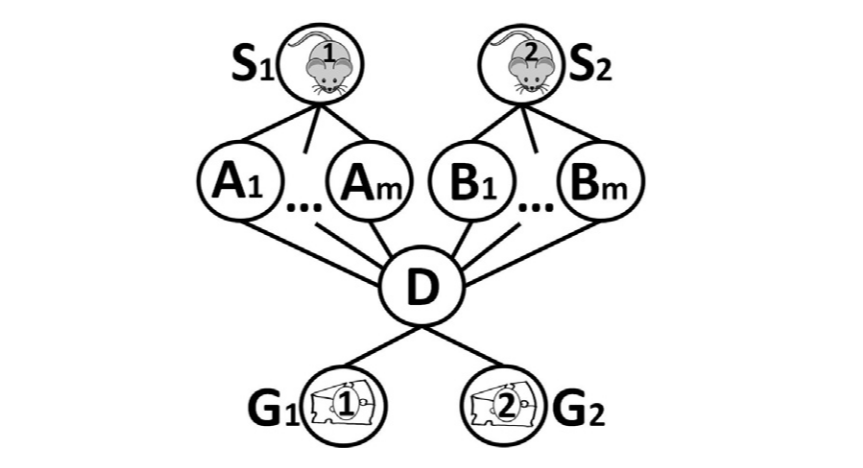
\includegraphics[width=\textwidth]{cbs_problem_example}
        \caption{Example MAPF instance illustrating potential conflicts between agents navigating a shared environment.}
        \label{fig:cbs_problem}
    \end{subfigure}
    \hfill
    \begin{subfigure}[t]{0.48\textwidth}
        \centering
        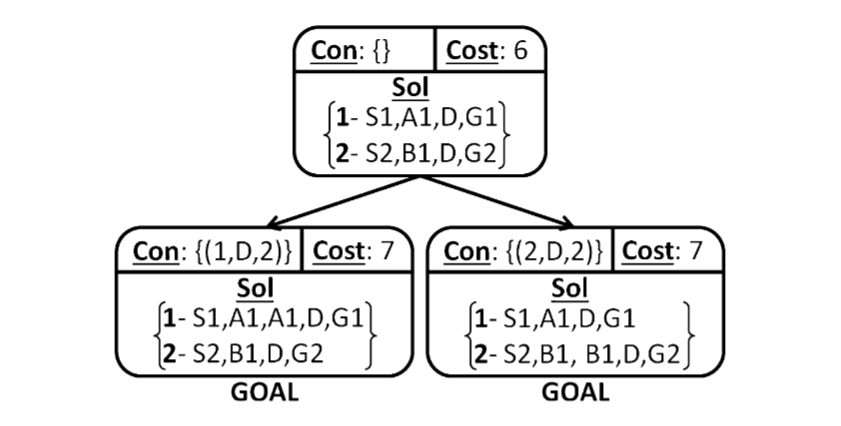
\includegraphics[width=\textwidth]{cbs_conflict_tree}
        \caption{Conflict Tree expansion in CBS, where conflicts are resolved by branching over alternative constraints.}
        \label{fig:cbs_conflict_tree}
    \end{subfigure}

    \caption{Overview of CBS. (a) A MAPF instance in which independently planned paths may lead to conflicts. (b) High-level Conflict Tree used by CBS to systematically resolve conflicts through constraint generation. Adapted from \cite{sharon2015conflict}.}
    \label{fig:cbs_overview}
\end{figure}

The high-level search maintains a Conflict Tree (CT), illustrated in Figure~\ref{fig:cbs_overview}\subref{fig:cbs_conflict_tree}, where each node corresponds to a set of constraints and associated individual paths. When a conflict is detected, the corresponding CT node is expanded by generating alternative constraint sets, each prohibiting one of the conflicting agents from performing the conflicting action. While this mechanism guarantees completeness and optimality under standard cost formulations, the number of conflicts and CT nodes may grow exponentially in the worst case, motivating several extensions to improve scalability.

At the low level, each agent computes a shortest path subject to a set of constraints. Recent extensions of CBS adopt Safe Interval Path Planning (SIPP) as the low-level planner in order to handle continuous time. This combination, commonly referred to as Continuous-Time CBS (CCBS), integrates SIPP into the CBS framework to enable optimal planning without discretizing time \cite{andreychuk2021ccbs, phillips2011sipp}. SIPP operates by representing, for each spatial location, intervals of time during which the location is safe to occupy, allowing waiting actions and motion durations to be handled efficiently under temporal constraints. This integration makes CBS particularly well suited for domains where temporal feasibility plays a central role \cite{phillips2011sipp}.



Several other variants of CBS have been proposed to address these limitations:
\begin{itemize}
    \item \textbf{ECBS:} Bounded-suboptimal CBS introduces focal search to trade optimality for efficiency, allowing solutions within a predefined suboptimality bound \cite{bar2014suboptimal}.
    
    \item \textbf{CBSH:} Heuristic-guided CBS augments the high-level search with admissible heuristics that estimate the cost of unresolved conflicts, significantly reducing the size of the conflict tree while preserving optimality \cite{felner2018adding}.
    
    \item \textbf{CBSH-RTC:} CBS variant with symmetry reasoning mitigate the combinatorial explosion of collision resolutions by identifying and pruning pairwise symmetric path combinations, substantially improving scalability and search efficiency. \cite{li2021realtime}.
\end{itemize}

Overall, CBS and its variants exemplify a conflict-driven coordination paradigm, in which interactions between agents are explicitly detected and resolved through constraint generation at the high level.

\subsubsection{Contrasting Centralized Coordination Strategies}
\label{subsubsec:tea_cbs_comparison}
\hspace{\parindent}
Although both TEA* and CBS are centralized approaches to multi-agent path finding, they embody fundamentally different coordination strategies. CBS follows a conflict-resolution paradigm, in which agents initially plan independently and conflicts are detected and resolved through constraint generation at a higher level. As a result, coordination emerges from the iterative refinement of individual plans in response to detected interactions.

In contrast, TEA* adopts a conflict-avoidance strategy by reserving spatial resources across discrete time layers, TEA* prevents conflicts by construction, rather than detecting and resolving them after paths have been generated. These contrasting design choices lead to different trade-offs in terms of computational complexity, solution optimality, and suitability for online execution, motivating their joint analysis in applied fleet management scenarios.



\subsection{Hybrid Coordination}
\label{subsec:hybrid_mapf}
\hspace{\parindent}
Hybrid MAPF approaches seek to combine elements of decentralized and centralized coordination in order to leverage the advantages of both paradigms. Typically, these approaches adopt a hierarchical structure, in which high-level coordination decisions are made centrally, while lower-level planning or execution decisions are delegated to individual agents, as illustrated in Figure~\ref{fig:hybrid_architecture}.

\begin{figure}[H]
    \centering
    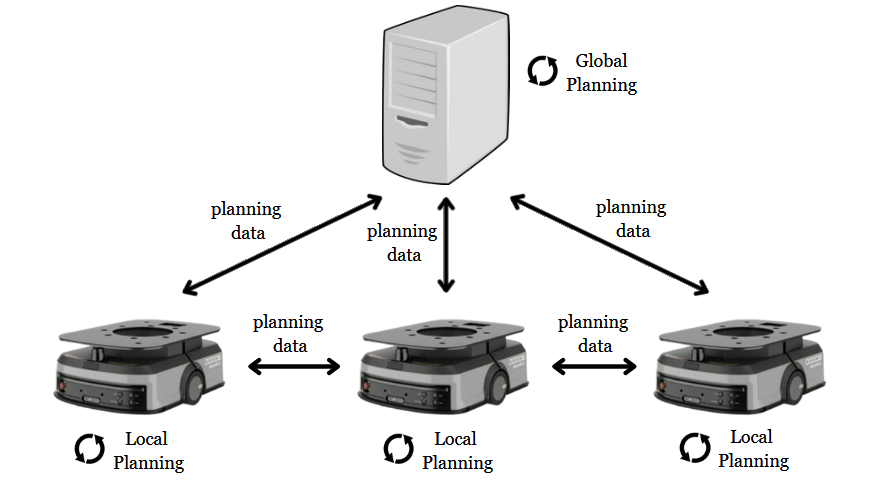
\includegraphics[width=0.8\textwidth]{hybrid_architecture}
    \caption{Illustration of a hybrid coordination architecture combining centralized decision-making at higher levels with decentralized planning or execution at the agent level.}
    \label{fig:hybrid_architecture}
\end{figure}


The motivation for hybrid coordination lies primarily in scalability. By abstracting parts of the problem or limiting centralized planning to higher-level decisions, hybrid approaches aim to reduce the computational burden associated with fully centralized coordination, while still preserving some degree of global consistency \cite{sang2021hybrid}.

Despite their potential benefits, hybrid and hierarchical approaches introduce additional complexity and may compromise theoretical guarantees. In particular, the separation between planning layers can lead to suboptimal solutions or coordination failures in complex or highly constrained environments. As such, hybrid paradigms are often tailored to specific application domains and system architectures.

Several representative approaches illustrate this hybrid coordination paradigm. Hierarchical MAPF methods employ centralized planning at a coarse level, such as region or waypoint assignment, while delegating fine-grained path planning to individual agents \cite{standley2010finding}. Other hybrid strategies rely on centralized global guidance combined with decentralized local execution, allowing agents to react autonomously to local disturbances while respecting global coordination constraints \cite{sang2021hybrid}. Region-based coordination approaches further reduce complexity by enforcing centralized constraints at the level of areas or traffic corridors, while allowing agents to plan locally within these regions \cite{zhang2021, leet2022}.




\subsection{Learning-Based Coordination}
\label{subsec:learning_mapf}
\hspace{\parindent}
More recently, learning-based approaches have been explored as an alternative paradigm for multi-agent coordination and path planning. These methods typically rely on machine learning techniques, such as reinforcement learning or imitation learning, to learn coordination policies from data rather than explicitly computing plans through search or optimization.

Learning-based coordination is motivated by the potential to generalize across environments and to adapt to complex, dynamic scenarios. In multi-agent settings, learning-based methods have been applied to collision avoidance, cooperative navigation, and decentralized decision-making \cite{junyan2020exploration, kulathunga2021learning}.

Representative examples of learning-based coordination include decentralized multi-agent reinforcement learning approaches, where agents learn local navigation and collision avoidance policies through interaction with the environment and other agents, without relying on explicit global planning \cite{everett2021collision}. Such methods emphasize scalability and adaptability, but typically lack formal guarantees.

Another prominent line of work combines classical MAPF planners with learning-based components. In these hybrid approaches, learning is used to guide heuristic selection, conflict resolution, or priority assignment within search-based planners, improving efficiency while preserving the underlying planning structure \cite{junyan2020exploration}.

Despite promising results, learning-based approaches face significant challenges in the context of MAPF. These include the need for large amounts of training data and the difficulty of providing strong guarantees regarding safety, completeness, or optimality. As a result, learning-based coordination is often considered complementary to classical MAPF methods rather than a direct replacement, particularly in safety-critical fleet management applications.

% --------------------------------
% --------------------------------
\section{Agent Prioritization Heuristics}
\label{sec:agent_prioritization}
\hspace{\parindent}
Prioritized planning constitutes an important class of MRPP approaches, particularly in centralized
settings where robots are planned sequentially according to a predefined priority ordering. In this
paradigm, higher-priority robots reserve their paths first, while lower-priority robots must plan
around the space-time constraints introduced by previously planned robots. Although this
decomposition makes the planning problem more tractable, it also makes the resulting solution highly
dependent on the selected ordering. Different priority permutations can lead to different levels of
feasibility, solution quality and computational effort~\cite{ma2019searching,zhang2022learning}.

The importance of priority assignment has therefore motivated several heuristic, randomized,
adaptive, and learning-based strategies for selecting or modifying robot orderings. As highlighted
by recent surveys on prioritised multi-robot path planning, no single priority rule is consistently
superior across all environments and task configurations~\cite{machines2023survey}. Instead,
performance depends strongly on factors such as robot distribution, path length, local density,
environmental bottlenecks, and the degree of interaction between robots. This motivates the use of
diverse prioritization criteria rather than relying on a single fixed ordering strategy.

\subsection{Randomized Strategies}
\hspace{\parindent}
A simple way to reduce the sensitivity of prioritized planning to robot ordering is to evaluate
multiple priority permutations. Bennewitz, Burgard and Thrun~\cite{bennewitz2002finding} explore
this idea by modifying priority schemes through a hill-climbing process, allowing the planner to
search for better orderings without enumerating all possible permutations.

Randomized orderings are also commonly used in MAPF as baselines or restart mechanisms
\cite{ma2019searching,zhang2022learning}. Although they can help escape poor deterministic
orderings, they do not provide an explicit criterion for why a given ordering should be effective.

\subsection{Distance and Path Length Heuristics}
\hspace{\parindent}
A common family of prioritization heuristics assigns priority according to geometric distance or estimated path length. These heuristics are attractive because they are
computationally lightweight and can be computed before the space-time planning stage.

Van den Berg and Overmars~\cite{vandenberg2005prioritized} use a roadmap-distance priority
criterion in which robots farther from their targets are given higher priority. The intuition is
that robots requiring longer movements are more likely to traverse a larger portion of the shared
environment and may therefore benefit from being planned before the roadmap becomes constrained by
reservations from other robots.

However, distance and path length rules only approximate coordination difficulty, since they do not explicitly capture the interaction structure of the problem, making them less reliable in bottlenecked or highly coupled environments.

\subsection{Local Density Heuristics}
\hspace{\parindent}
Another class of prioritization methods uses the local surroundings of each robot as an estimate of
planning difficulty. The underlying assumption is that robots located in more cluttered or locally
constrained regions may have fewer immediate movement options and may therefore benefit from
being planned earlier.

Wu, Bhattacharya and Prorok~\cite{wu2019pathprospects} discuss two surroundings-based priority
rules. The first, \emph{Naive Surroundings}, counts the number of original obstacles within a fixed
range around each robot and gives higher priority to robots with more crowded surroundings. This
heuristic is considered naive because it only counts nearby obstacles and does not account for the
coupling between robot mobility and the environment. The second, \emph{Coupled Surroundings},
extends this idea by counting effective obstacles, thereby considering whether nearby obstacles
actually restrict the feasible motion of the robot.

These heuristics show that local spatial context can be used as a lightweight priority signal, although their effectiveness depends on how neighbourhoods are defined and on whether the resulting density measure reflects actual motion constraints. Euclidean neighbourhoods provide a simple geometric estimate of local density, while neighbourhoods defined over the roadmap can better capture environmental connectivity, especially when obstacles make geometric distance differ from graph distance.

\subsection{Environment Heuristics}
\hspace{\parindent}
Several prioritization strategies exploit structural properties of the environment, since paths
through constrained or highly shared regions may become harder to accommodate after other
reservations have been introduced.

A representative example is the \emph{Path Prospects} heuristic proposed by Wu, Bhattacharya and
Prorok~\cite{wu2019pathprospects}, which prioritizes robots according to the number of meaningful
route alternatives available between their current position and target. Robots with fewer
alternatives are considered more constrained and are planned earlier, since delaying them may make
their paths harder to accommodate after reservations from other robots have been introduced.

Another strategy assigns priority according to the expected use of shared infrastructure. For
example, ter Mors~\cite{termors2011evaluating} considers an ordering criterion based on the busiest
parts of the infrastructure, where agents that depend on highly used segments are prioritized
earlier. In this case, priority depends not only on the individual route of an agent, but also on the
expected congestion along that route.

These approaches assign priority according to how constrained or critical each route is within the
shared environment. In particular, they attempt to capture whether a robot depends on limited route
alternatives or on shared infrastructure that may become difficult to access once other reservations
have been introduced.

\subsection{Conflict and Interaction Prioritization}
\hspace{\parindent}
Methods based on conflict information use interactions between agents competing for the same
vertices, edges, or temporal resources as a source of priority information. Although CBS is not
itself a prioritization heuristic, it demonstrates the importance of conflict information in MAPF by
detecting conflicts between paths and resolving them through alternative constraint
sets~\cite{sharon2015conflict}. This makes conflicts a useful signal for identifying coupled agents
and difficult coordination decisions.

An indirect form of interaction awareness is considered by ter Mors~\cite{termors2011evaluating},
where one heuristic evaluates the quality of a context-aware route using the ratio 
\[
q_i = \frac{c_i}{\ell_i}
\]
, where \(c_i\) is the cost of the context-aware plan of agent \(i\), and \(\ell_i\) is the length of
its shortest path. Higher values of \(q_i\) indicate that the route is more strongly affected by
existing plans or shared-resource usage, making this criterion an indirect measure of interaction
pressure~\cite{termors2011evaluating}.

Overall, while conflicts can provide useful indicators of agent interaction, the literature does not
appear to provide many explicit prioritization heuristics that use predicted space-time conflicts as
a lightweight pre-planning score for constructing an initial priority ordering.

\subsection{Rescheduling and Adaptive Priority Adjustment}
\hspace{\parindent}
Priority orderings do not necessarily remain fixed throughout the planning process. In rescheduling
methods, feedback from previous planning attempts, such as failures, is used to adjust the ordering during replanning.

Regele and Levi~\cite{regele2006cooperative} propose a heuristic priority-adjustment mechanism in
which robots initially have low priority values, which are increased when planning becomes difficult
or unsuccessful. Andreychuk and Yakovlev~\cite{andreychuk2018two} later simplify this idea through
deterministic rescheduling, where a robot that fails to find a route is assigned maximum priority in
the next planning attempt. This follows the assumption that failure indicates strong dependence on
the current ordering.

Other adaptive strategies modify only part of the priority order. Local priority adjustment focuses
on robots involved around a deadlock region, while priority tuning increases the priority of robots
whose routes are least optimal and repeats this process until no significant improvement is
obtained~\cite{machines2023survey}. Overall, these methods show that replanning feedback can be
used to refine priority decisions instead of treating each ordering as independent.

\subsection{Learning Priority Orderings}
\hspace{\parindent}
Learning priority approaches provide an alternative to manually defined prioritization rules. Instead
of selecting a fixed heuristic a priori, Zhang et al.~\cite{zhang2022learning} propose learning
priority orderings for prioritized MAPF from training data. Their method first generates candidate
solutions by running prioritized planning with different orderings, including heuristic and random
priority assignments, and then uses the best-performing orderings as supervision for learning.

The authors consider two learning formulations. The first learns a total priority ordering, where
all agents are ranked before planning. The second learns partial priority relations between agents,
allowing the method to focus on the ordering decisions that are more relevant to solution quality.
The learned models use features related to start-goal distances, path alternatives, and potential
interactions between agents, combining several signals that are often treated separately in
handcrafted heuristics.

Although this allows priority rules to be inferred from data, learning-based methods require
training instances, feature design, and generalization across maps and problem distributions.
Therefore, handcrafted heuristics remain relevant when interpretability, low computational cost, and
direct control over the prioritization criterion are important.


% --------------------------------

\section{Fleet Coordination System}
\label{sec:criis_architecture}
\hspace{\parindent}
This section describes the architecture of the CRIIS fleet coordination system, which is designed as a centralized coordination framework built around TEA*, complemented with supervision and graph-processing mechanisms to handle real-world scenarios \cite{matos2025criis}. The system is implemented on top of the Robot Operating System (ROS), which provides the communication middleware and execution infrastructure supporting both centralized coordination and distributed robot control.

The architecture follows a modular design that separates global coordination responsibilities from local robot control. As illustrated in Figure~\ref{fig:criis_high_level}, at a high level, the system is composed of two main components. The \emph{Central Coordination Module} is responsible for global planning, supervision, and coordination, maintaining a global view of the environment and the fleet state. In contrast, the \emph{Agent Control Module}, instantiated on each robot, is responsible for executing the received plans, interfacing with the robot's navigation stack, and providing execution feedback to the central supervisor \cite{matos2025criis}.


\begin{figure}[H]
    \centering
    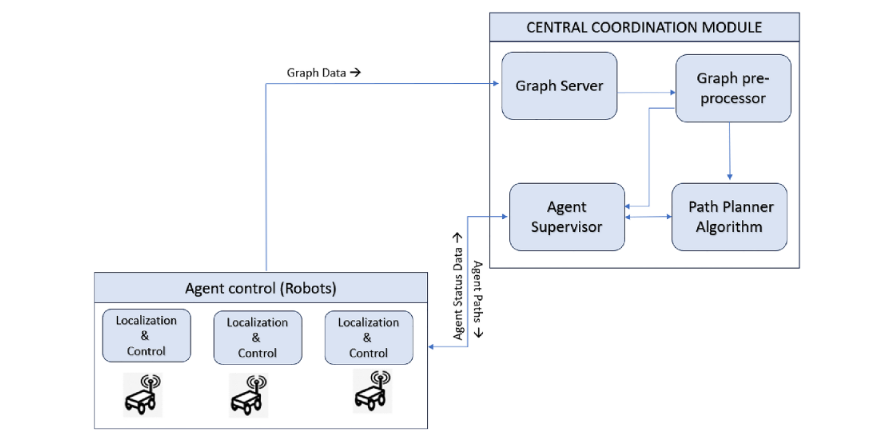
\includegraphics[width=0.85\textwidth]{matos.png}
    \caption{High-level architecture of the CRIIS fleet coordination system \cite{matos2025criis}.}
    \label{fig:criis_high_level}
\end{figure}

The remainder of this section focuses on a detailed description of the Central Coordination Module and its internal components.


\subsection{Central Coordination Module}
\label{subsec:central_coordination_module}
\hspace{\parindent}
The Central Coordination Module is responsible for global decision-making and coordination across the robotic fleet. It maintains a centralized representation of the environment and agent states, computes coordinated plans, and supervises execution\cite{matos2025criis}.

As summarized in Figure~\ref{fig:criis_sequence_diagram}, this module comprises four core components: the Graph Server, the Graph Pre-Processor, the Path Planner, and the Supervisor. Interaction with the robots' navigation systems is mediated through a Navigation Handler, which provides an abstraction layer for plan dispatch and execution feedback.

\begin{figure}[H]
    \centering
    
\includegraphics[width=0.95\textwidth]{seqDiagram}
    \caption{Sequence diagram of the CRIIS fleet coordination workflow.}
    \label{fig:criis_sequence_diagram}
\end{figure}



\subsubsection{Graph Server}
\hspace{\parindent}
The Graph Server is responsible for storing and providing access to the global navigation graph shared by all agents in the fleet. This graph encodes the topological structure of the environment, including nodes, directed edges, and their associated traversal costs. In the CRIIS fleet coordination system, these costs are expressed in temporal terms, enabling time-aware planning and synchronization among agents \cite{matos2025criis}.

Additionally, the Graph Server exposes a query interface that allows other components, namely the Path Planner, to retrieve graph topology, edge attributes, and metadata required for coordination. By decoupling graph management from planning logic, the system promotes modularity and facilitates future extensions, such as dynamic cost updates or graph augmentation strategies.

\subsubsection{Graph Pre-Processor}
\hspace{\parindent}
The Graph Pre-Processor operates during an offline configuration phase and augments the raw navigation graph with information required for multi-robot coordination, transforming a purely geometric representation into a coordination-aware graph \cite{matos2025criis}. Its responsibilities include identifying footprint-related constraints, such as parallel edges that cannot be safely occupied simultaneously, and detecting critical shared resources (choke points) like narrow corridors or doorways that are prone to congestion and deadlocks.

Additionally, since TEA* advances time in discrete steps associated with edge traversals, the pre-processor performs edge discretization and normalization according to a global temporal resolution. This ensures consistent traversal times across the graph, improving temporal alignment between agents and enabling more accurate space--time reasoning during planning, thereby reducing synchronization errors and unnecessary replanning \cite{matos2025criis}.



\subsubsection{Path Planner}
\hspace{\parindent}
The Path Planner is the core decision-making component responsible for computing coordinated, collision-free trajectories for the entire fleet. In the CRIIS system, this functionality is implemented using the TEA* algorithm \cite{matos2025criis}.

Planning requests include the current symbolic positions and target goals of all agents. Upon receiving a request, the Path Planner retrieves the navigation graph and associated traversal costs from the Graph Server and computes time-consistent sequences of edges for each agent. By reasoning over a shared space--time representation, the planner can explicitly account for interactions between agents, reserving graph resources over time and preventing conflicts through temporal exclusion mechanisms.

The centralized nature of the Path Planner enables globally coherent solutions, particularly in environments with shared resources or high robot density. This approach allows conflicts to be resolved at planning time rather than during execution, reducing the likelihood of deadlocks, emergency stops, or excessive local replanning \cite{matos2025criis}.


\subsubsection{Navigation Handler}
\hspace{\parindent}
The Navigation Handler serves as the integration layer between the centralized coordination logic and the robots' low-level navigation systems. It exposes an API that supports navigation requests, plan dispatch, translation of symbolic graph-based edge sequences into commands compatible with the robot navigation stack, and continuous monitoring of execution progress.

In particular, the Navigation Handler provides a planning service through which a robot can be requested to navigate to a given target vertex. When this service is called, the Navigation Handler forwards the request to the Supervisor, which in turn invokes the Path Planner to compute a feasible path within the shared graph representation. Once the resulting plan is received, the Navigation Handler translates the symbolic sequence of graph edges into navigation commands executable by the robot.

During execution, the Navigation Handler collects feedback such as the current symbolic state, edge completion status, and execution delays, and reports this information to the Supervisor. By isolating execution-specific concerns from planning logic, it enhances system modularity and allows the coordination framework to remain agnostic to the underlying robot platforms and navigation implementations \cite{matos2025criis}.

\subsubsection{Supervisor}
\hspace{\parindent}
The Supervisor is responsible for orchestrating the overall coordination loop by closing the feedback cycle between planning and execution. It aggregates execution feedback provided by the Navigation Handler, monitors the progress of each agent, and maintains a global view of the system state \cite{matos2025criis}.

Based on this information, the Supervisor detects abnormal or unexpected conditions, such as execution delays, deviations between planned and executed trajectories, or emerging conflicts caused by dynamic disturbances. When such situations are identified, the Supervisor triggers replanning requests to the Path Planner.

This supervision mechanism is a key contributor to system robustness under real-world uncertainty, including variable execution times, communication latency, and dynamic obstacles. By enabling adaptive replanning while preserving centralized coordination, the Supervisor ensures that the fleet can maintain safe and efficient operation even when assumptions made at planning time are violated \cite{matos2025criis}.

\section{Summary}
\label{sec:soa_summary}
\hspace{\parindent}
This chapter reviewed the main coordination paradigms and algorithmic approaches to MAPF, with particular emphasis on centralized planning methods. While decentralized and learning-based approaches offer scalability and adaptability, their limited guarantees regarding safety, predictability, and solution quality restrict their applicability in tightly coordinated fleet management scenarios.

Motivated by these constraints, the CRIIS fleet coordination system adopts a centralized, time-aware coordination architecture that explicitly reasons about agent interactions and execution timing. By integrating TEA* within a broader framework that includes graph preprocessing, supervision, and execution monitoring, CRIIS bridges the gap between theoretical MAPF formulations and the practical requirements of real-world robotic fleets, such as execution uncertainty, communication delays, and physical interaction constraints.

A central design choice in CRIIS is the use of sequential, prioritized planning, which enables
responsive and scalable coordination but introduces a strong dependence on robot ordering.
Although the impact of priority ordering is recognized in the literature, robot prioritization has
received comparatively less systematic attention than the underlying MAPF algorithms themselves.
This observation motivates the heuristic design and multi-ordering strategies developed in the
following chapters.